% Exam Template for UMTYMP and Math Department courses
%
% Using Philip Hirschhorn's exam.cls: http://www-math.mit.edu/~psh/#ExamCls
%
% run pdflatex on a finished exam at least three times to do the grading table on front page.
%
%%%%%%%%%%%%%%%%%%%%%%%%%%%%%%%%%%%%%%%%%%%%%%%%%%%%%%%%%%%%%%%%%%%%%%%%%%%%%%%%%%%%%%%%%%

% These lines can probably stay unchanged, although you can remove the last
% two packages if you're not making pictures with tikz.
\documentclass[12pt]{exam}
\RequirePackage{amssymb, amsfonts, amsmath, latexsym, verbatim, xspace, setspace}
\RequirePackage{tikz, pgflibraryplotmarks}

% By default LaTeX uses large margins.  This doesn't work well on exams; problems
% end up in the "middle" of the page, reducing the amount of space for students
% to work on them.
\usepackage[margin=1in]{geometry}

% To insert a picture, one should define the graphics path first.
\usepackage{graphicx}
\graphicspath{ {./} }

% Here's where you edit the Class, Exam, Date, etc.
\newcommand{\class}{Grade 11 Mathematics}
\newcommand{\term}{Springs Boys High School}
\newcommand{\examnum}{Controlled Test Paper 2}
\newcommand{\examdate}{June 2022}
\newcommand{\markstotal}{100 Marks}
\newcommand{\duration}{2 hours}
\newcommand{\moderator}{Mr. Ratsela \& Mrs. Reynecke}
\newcommand{\examinator}{Mr. Wessels}

% For an exam, single spacing is most appropriate
\singlespacing
% \onehalfspacing
% \doublespacing

% For an exam, we generally want to turn off paragraph indentation
\parindent 0ex

% Hide points in document. Points have to be hard-coded into questions.
\nopointsinmargin
\pointformat{}

% Change Enumeration
\usepackage[shortlabels]{enumitem}



\renewcommand\partlabel{\thepartno.}

\renewcommand{\questionlabel}{\thequestiontitle.}
\renewcommand{\thepartno}{\thequestiontitle.\arabic{partno}}
\renewcommand{\thesubpart}{\thequestiontitle.\arabic{partno}.\arabic{subpart}}


%\renewcommand\partlabel{(*)}


\begin{document} 

% These commands set up the running header on the top of the exam pages
%\pagestyle{head}
%\firstpageheader{}{}{}
%\runningheader{\class}{Page \thepage\ of \numpages}{\examdate}
%\runningheadrule



\pagestyle{headandfoot}
\firstpageheader{}{}{}
%\firstpagefootrule
\firstpagefooter{}{Page \thepage\ of \numpages}{}
\runningheader{\class}{\examdate}{\examnum}
\runningfooter{}{Page \thepage\ of \numpages}{}



\begin{center}
\includegraphics[width=4cm,height=4cm]{emblem.jpg}
\end{center}

\begin{center}

\textbf{\term} \\

\textbf{\class}\\

\textbf{\examnum} \\

\textbf{\examdate} \\


\end{center}


\begin{flushleft}
\begin{tabular}{p{3in} r l}


\end{tabular}\\
\end{flushleft}

\begin{flushleft}
\begin{tabular}{p{10cm} p{5cm}}

\textbf{Examinator: \examinator} &  \textbf{Total: \markstotal} \\
\textbf{Moderator: \moderator} & \textbf{Duration: \duration} \\
\textbf{} & ${}$ \\
${}$ &  \\



\textbf{Name:} \makebox[2.65in]{\hrulefill} & ${}$\\

\smallskip

\textbf{Teacher:} \makebox[2.5in]{\hrulefill} & ${}$\\

\end{tabular}
\end{flushleft}

\smallskip

\vspace{0.5cm}

\rule[1ex]{\textwidth}{.1pt}

\medskip

\quad \textbf{Instructions:}

\begin{itemize}
\item Answer all the questions.
\item Write neatly and legibly.
\item Write your name at the top of your answer sheet.
\item Indicate your class teachers' code at the top of your answer sheet.
\item Label the questions according to the numbering used on the question paper.
\item Leave answers in simplest root form or two decimal places unless otherwise stated.
\item Show all calculations. Answer only will not necessarily get full marks.
\item Clearly indicate your class and write your name on your question paper.
\item The use of a non-programmable calculator is permitted, unless otherwise stated.
\item This assessment contains \numpages\ pages (including the cover page) and \numquestions\ questions.
\end{itemize}

\rule[1ex]{\textwidth}{.1pt}

\hfill

\vspace{0.5cm}

%\begin{center}
%\cellwidth{3em}
%\gradetablestretch{2}
%\vqword{Problem}
%\addpoints % required here by exam.cls, even though questions haven't started yet.	
%\gradetable[h]%[pages]  % Use [pages] to have grading table by page instead of question
%\end{center}

\newpage % End of cover page

%%%%%%%%%%%%%%%%%%%%%%%%%%%%%%%%%%%%%%%%%%%%%%%%%%%%%%%%%%%%%%%%%%%%%%%%%%%%%%%%%%%%%
%
% See http://www-math.mit.edu/~psh/#ExamCls for full documentation, but the questions
% below give an idea of how to write questions [with parts] and have the points
% tracked automatically on the cover page.
%
%%%%%%%%%%%%%%%%%%%%%%%%%%%%%%%%%%%%%%%%%%%%%%%%%%%%%%%%%%%%%%%%%%%%%%%%%%%%%%%%%%%%%

\begin{questions}

\newpage

% Question with parts



\addpoints
\question \textbf{Question 1} \hfill \textbf{[30]}

\vspace{0.5cm}

In the diagram below, $ABCD$ is a parallelogram with coordinates $A(1;2)$, $B(7,2)$, $D(5;5)$ and $C(x;y)$.

\begin{center}
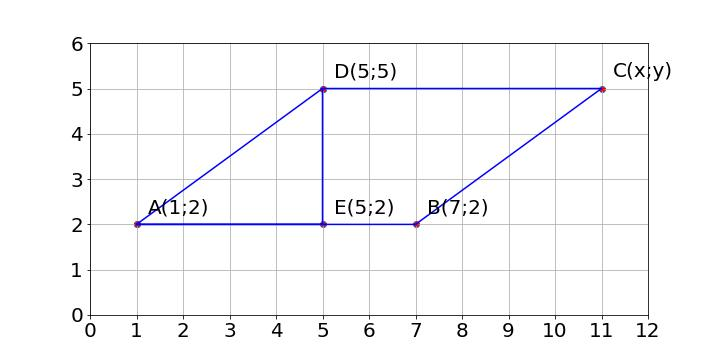
\includegraphics[width=11cm, height=7cm]{parallelogram.jpg}
\end{center}

\begin{parts}

%\setcounter{partno}{1} %% Setting the counter to 1

\vspace{0.5cm}

\part[4] Calculate the length of segments $AB$ and $DE$. \hfill (4)

\vspace{0.5cm}

\part[4] Calculate the length of the segment $AD$. \hfill (4)

\vspace{0.5cm}

\part[4] Determine the equation of the line passing through $B$ and $C$. \hfill (4)

\vspace{0.5cm}

\part[2] Determine the equation of the line passing through $D$ and $C$. \hfill (2)

\vspace{0.5cm}

\part[3] Use your answers in 1.3 and 1.4 to determine the coordinate of $C$. \hfill (3)

\vspace{0.5cm}

\part[3] Show that $AC$ and $BD$ have the same midpoint. \hfill (3)

\vspace{0.5cm}

\part[4] Show that the diagonals of $ABCD$ do not intersect at a right angle. \hfill (4)

\vspace{0.5cm}

\part[3] Use your answer from 1.1 to calculate the area of the parallelogram. \hfill (3)

\vspace{0.5cm}

\part[3] Determine the inclination angle of the line passing through $A$ and $D$. \hfill (3)

\vspace{0.5cm}

\end{parts}



\pagebreak



\addpoints
\question \textbf{Question 2} \hfill \textbf{[43]}

\begin{parts}

%\setcounter{partno}{1} %% Setting the counter to 1

\vspace{0.5cm}

\part Without using a calculator, simplify the following expression to a single ratio:

\vspace{0.5cm}

\begin{subparts}

    \subpart[6] \begin{LARGE} $\frac{ \tan(180^o - \theta) \sin(360^o + \theta) }{ \cos(180^o + \theta) \tan(360 - \theta) }$ \end{LARGE} \hfill (6)

	\vspace{0.5cm}
    
    \subpart[6] \begin{large} $\cos(315^o) \cos(405^o) + \sin(45^o) \sin(135^o)$ \end{large} \hfill (6)
	
\end{subparts}

\vspace{0.5cm}

\part Prove the following identities:

\vspace{0.5cm}

\begin{subparts}

    \subpart[6] \begin{LARGE} $ \frac{ ( \cos \theta - 1 )( \cos \theta + 1 ) }{ ( \sin \theta - 1 )( \sin \theta + 1 ) } =$ \end{LARGE} \begin{large} $ - \tan \theta $ \end{large} \hfill (6)

	\vspace{0.5cm}
    
    \subpart[5] \begin{LARGE} $ \frac{ 1-\sin \theta }{ \cos \theta }  = \frac{ \cos \theta }{ 1+ \sin \theta } $ \end{LARGE} \hfill (5)
	
\end{subparts}

\vspace{0.5cm}

\part Given coordinate $P(-4,y)$ and $\tan \theta > 0$;

\vspace{0.5cm}

\begin{subparts}

	\subpart[3] Construct a triangle in the relative quadrant to represent $\theta$. \hfill (3)
	
	\vspace{0.5cm}
	
	\subpart[3] Calculate \begin{large} $\cos (180^o - \theta)$. \end{large} \hfill (3)

\end{subparts}

\vspace{0.5cm}

\part The trigonometric function $g(x) = a \cdot \cos(k \cdot x) + q$ is sketched below:

\begin{center}
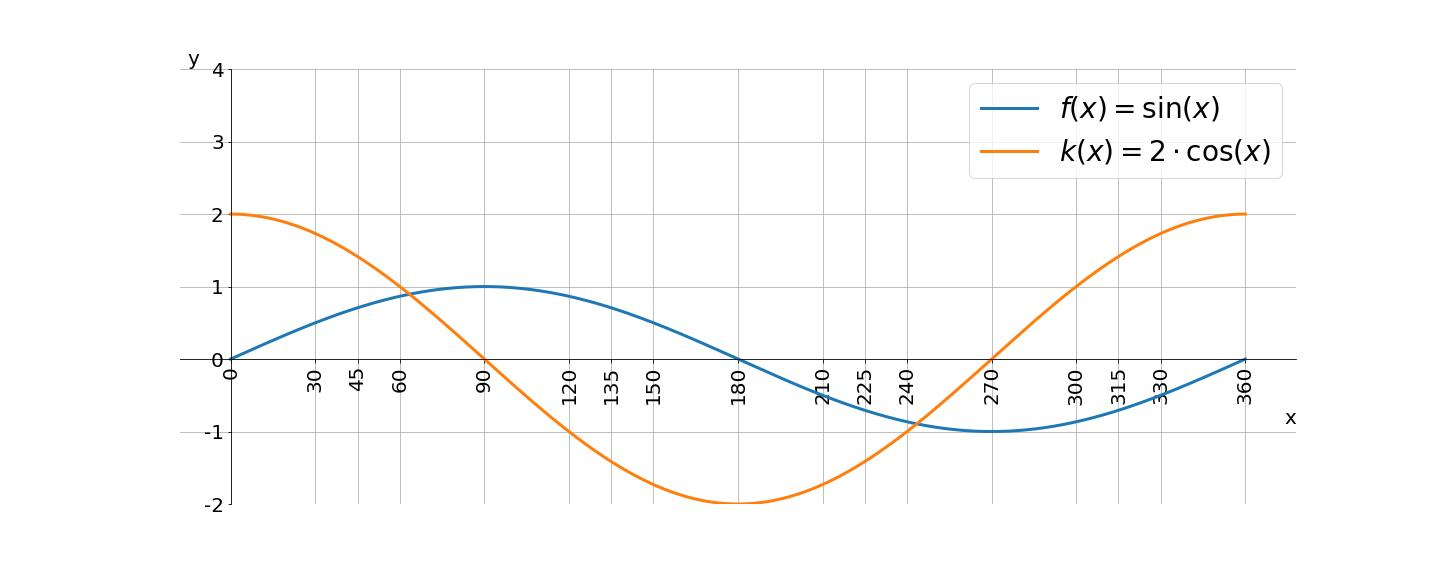
\includegraphics[width=15cm, height=6cm]{trigonometry.jpg}
\end{center}



\begin{subparts}
	
	\subpart[2] What is the domain of $g(x)$? \hfill (2)
		
	\vspace{0.5cm}
	
	\subpart[3] Write down the equation of the function $g(x)$. \hfill (3)
		
	\vspace{0.5cm}
	
	\subpart[3] If $h(x) = g(x)-1$, write down the and range of $h(x)$. \hfill (3)

\end{subparts}

\vspace{1cm}

\part Below are the graphs of $f(x)= \sin(x)$ and $k(x)=2 \cos(x)$:

\begin{center}
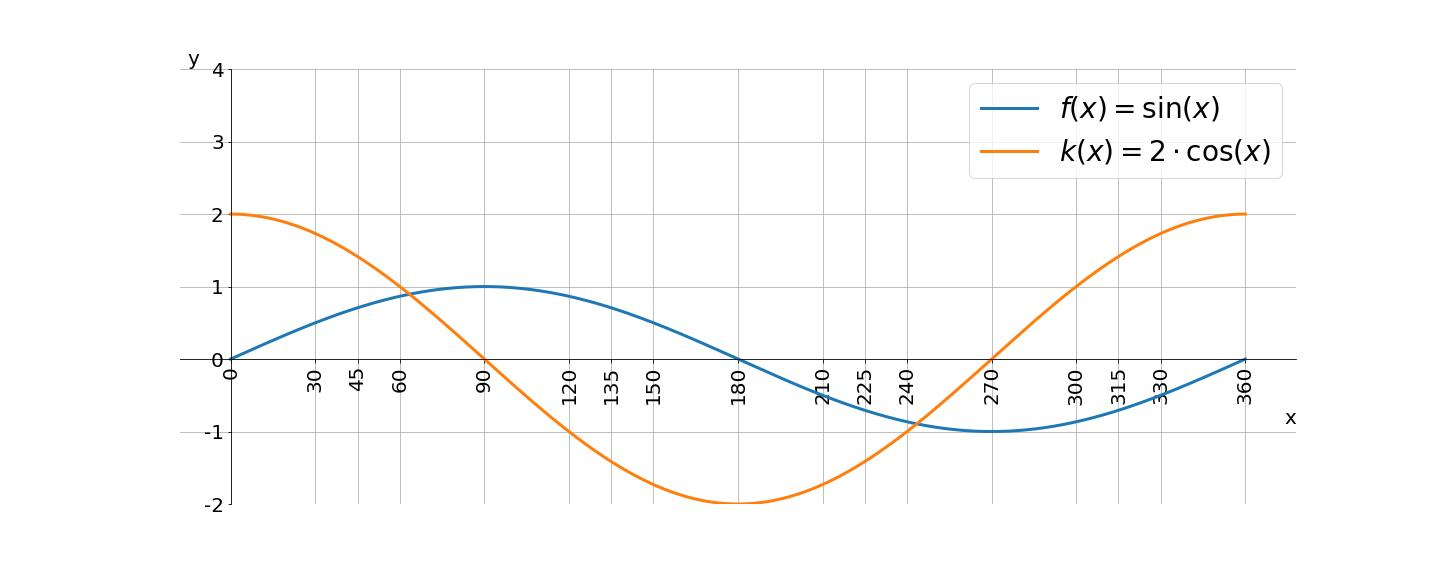
\includegraphics[width=15cm, height=6cm]{intersection.jpg}
\end{center}

\begin{subparts}

	\subpart[5] Determine the values of $x$ where the $f(x)=k(x)$. \hfill (5)

\end{subparts}

\end{parts}


\vspace{1cm}


\addpoints
\question \textbf{Question 3} \hfill \textbf{[28]}

\vspace{0.5cm}

\begin{parts}

\part In the diagram below, $BE$ and $CD$ are diameters of a circle with center $M$. Chord $AE$ is drawn to cut $CD$ at $F$. $AE \perp CD$ and $\hat{C} = x$.

\smallskip

\begin{center}
\includegraphics[width=7cm, height=7cm]{circle1.jpg}
\end{center}

\vspace{0.5cm}

\begin{subparts}

	\subpart[1] Give a reason why $AF=EF$. \hfill (1)
	
	\vspace{0.5cm}
	
	\subpart[4] Determine with reason the size of $\hat{M_1}$ in terms of $x$. \hfill (4)
	
	\vspace{0.5cm}
	
	\subpart[6] Prove that $AD$ is a tangent to the circle passing through $A$, $C$ and $F$ \hfill (6)

\end{subparts}

\vspace{0.5cm}

\part  In the diagram below, $APL \text{\space} || \text{\space} CB$ and $\hat{A_2} = \hat{B_2}$.


\begin{center}
\includegraphics[width=12.5cm, height=9cm]{circle2.jpg}
\end{center}

\begin{subparts}

	\subpart[6] Prove that $PAL$ is a tangent to circle $ABC$ \hfill (6)
	
	\vspace{0.5cm}
	
	\subpart[6] Prove that $AB$ is a tangent to the circle $ADP$ \hfill (6)
	
\end{subparts}


\vspace{0.5cm}

\part In the diagram below $O$ is the center of the circle, $OM \perp AB$, $ON \perp CD$, $AB = 60$ mm, $OM = 40$ mm and $ON = 30$ mm.


\begin{center}
\includegraphics[width=9cm, height=9cm]{circle3.jpg}
\end{center}

\begin{subparts}

	\subpart[2] Calculate the radius of the circle \hfill (2)
	
	\vspace{0.5cm}
	
	\subpart[3] Calculate the length of $CD$ \hfill (3)

\end{subparts}


\end{parts}



%	 \begin{center}
%	 \includegraphics[width=8cm, height=6cm]{question2.jpg}
%	 \end{center}

%    \begin{center}
%	 \begin{tabular}{ | p{7cm} | p{7cm} | }
%	 \hline
%	 Statement & Reason \\
%	 \hline
%	 ${}$ & ${}$ \\ 
%	 \hline 
%	 ${}$ & ${}$ \\ 
%	 \hline
%	 ${}$ & ${}$ \\ 
%	 \hline
%	 \end{tabular}
%	 \end{center}

\end{questions}
\end{document}